% --------------------------- INTRODUCTION ----------------------------
\section{Introduction}
\label{sec:intro}

Index rebalancing creates a recurring implementation problem for passive and enhanced-index investors. Once an index provider announces additions and deletions, benchmarked capital must trade in the same direction and over a narrow window. That demand pressure can move prices even when firm fundamentals are unchanged, the classic ``index effect'' of \textcite{shleifer-do-demand-curves-for-stocks-slope-down}. The effect has been documented for large global indices \parencite{lynch-new-evidence-s&p-500,afego-effects-of-changes-in-stock-index-composition} and is the empirical counterpart to the avoidable rebalancing drag estimated for benchmarked mandates \parencite{arnott-the-avoidable-cost-of-index-rebalancing}; the investment question is whether it can be forecast early enough, and cleanly enough, to be traded.

OSEBX is a useful laboratory because the index is important locally, liquid enough for institutional implementation, and transparent. Euronext selects roughly 50--80 names from the wider OSEAX universe twice per year using publicly described eligibility, turnover, free-float and sector rules \parencite{OSEBX-rule-book}. Figure~\ref{fig:idxeff} shows the economic motivation: from 2002 to 2023, future additions tended to outperform and future deletions tended to underperform before the effective date. The opportunity lies between the data cut-off date and the announcement date, when the relevant inputs are fixed but the official constituent list is not yet public.

\begin{figure}[H]
\centering
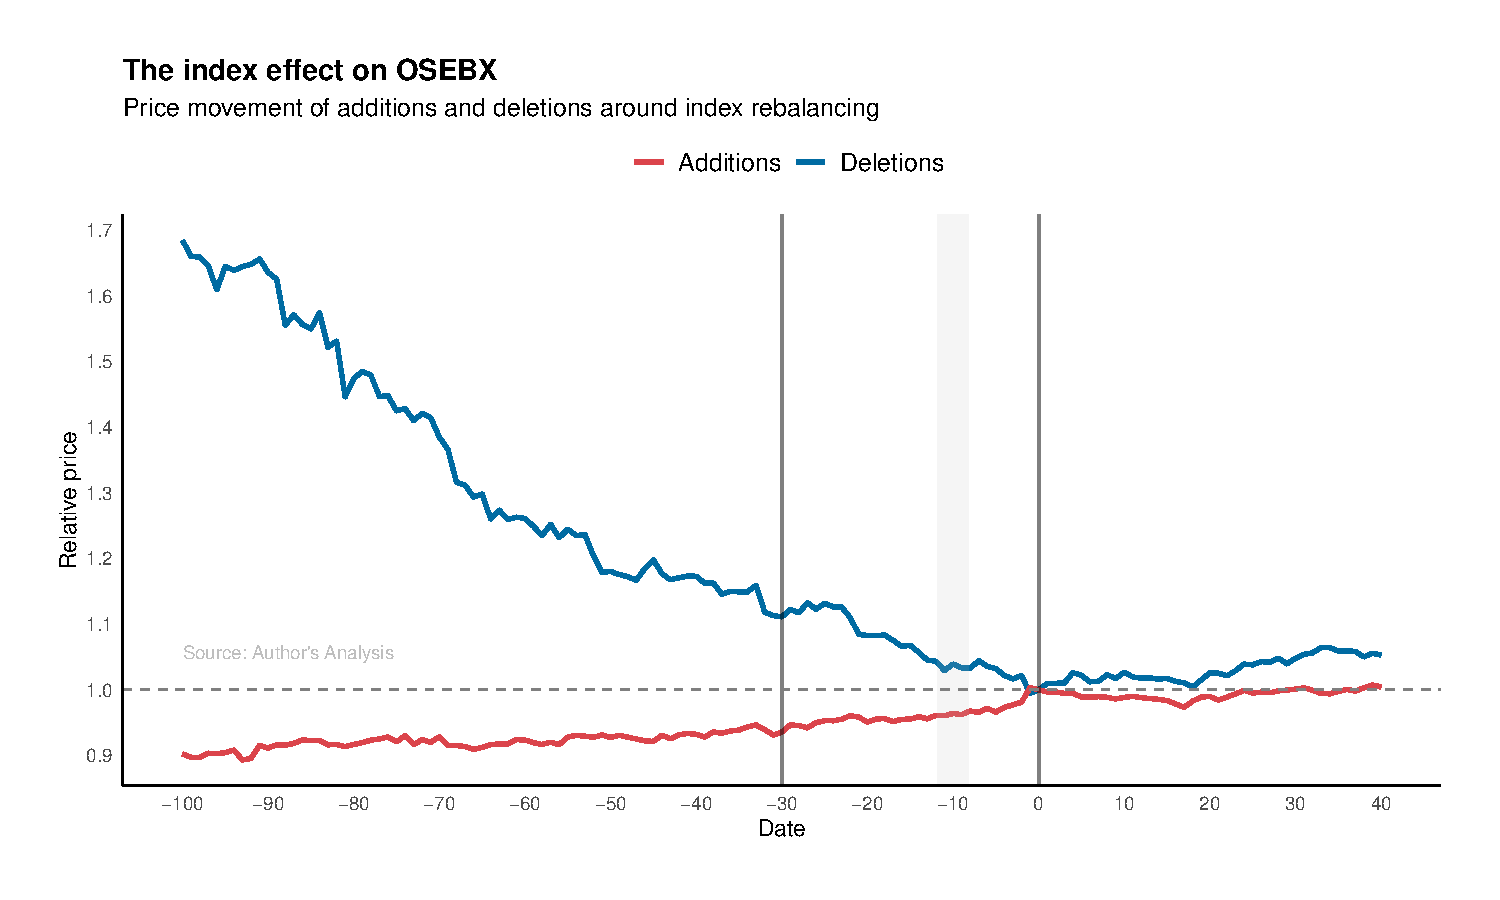
\includegraphics[width=0.8\linewidth]{images/index_plot_updated.pdf}
\caption{\textbf{OSEBX index effect, 2002--2023.} Average relative price paths for future additions and deletions around the effective date (day 0). Prices are Bloomberg VWAP series aggregated across historical rebalancing events.}
\label{fig:idxeff}
\end{figure}

The paper contributes a compact, implementable answer to three questions. First, can upcoming OSEBX membership be predicted out of sample using only rule-book information? Second, do the predictions survive transaction costs, short-borrow charges and monthly risk adjustment? Third, can the signal still matter inside the tighter constraints of an enhanced-index mandate, where active risk is capped by tracking error?

The answer is yes, with an important qualification. Machine learning can forecast OSEBX membership with very high headline accuracy, but the highest-accuracy model is also the least useful one: it simply predicts no change. I therefore treat the task as a portfolio-design problem rather than a pure classification problem. The proposed conditional threshold increases the density of addition and deletion signals, and the resulting XGBoost strategy is the only specification that remains economically meaningful after scaling into a 2\% annual tracking-error enhanced-index portfolio.

The contribution sits at the intersection of three literatures. First, the index-effect literature documents reliable price pressure around scheduled rebalances and motivates the trade idea. Second, an emerging strand of work applies machine learning to portfolio construction, showing that tree-based models can outperform linear baselines once features carry mild non-linearities or interactions \parencite{rouf-stock-market-prediction-using-machine-learning,goodell-artificial-intelligence-and-machine-learning-in-finance}. Third, the enhanced-indexing literature constrains active risk by tracking error and so penalises high-volatility overlays \parencite{ahmed-performance-of-enhanced-index-and-quantitative-equity-funds,nbim-from-passive-to-enhanced}. The novelty here is to fuse the three: a rule-book classifier whose loss function is reshaped to optimise a tracking-error-bounded portfolio rather than headline accuracy.
